\chapter{A Nonequilibrium Phase Transition}
\label{chapter5}

In an open system, the competition between unitary Hamiltonian evolution and dissipation can induce a dissipative phase transition for the steady state, as discussed for example in the case of spin systems by~\cite{phase_trans_spin_system}.
A phase transition is an important phenomenon in condensed-matter physics and can happens tuning one or more parameters of the Hamiltonian of the system. 

So far, we have studied the behaviour of 8, 12 and 16-sites chain varying the coefficient of dissipation rate $\gamma$. In this chapter, the behaviour of the chains under a variation of $J_z$ will be investigated.

First of all, we have analyzed the spin current under the variation of the coupling constant $J_z$. In fig.~\ref{fig:16sites_SpinCurrVaryingJz} the spin current for several values of $J_z$ is displayed. Some consideration can be made in regards to this plots.

%This behaviour is confirmed by the data obtained from QT method (fig.~\ref{fig:8sites_spinCurrVSJzQT}).

%\begin{figure}[H]
    %\centering
    %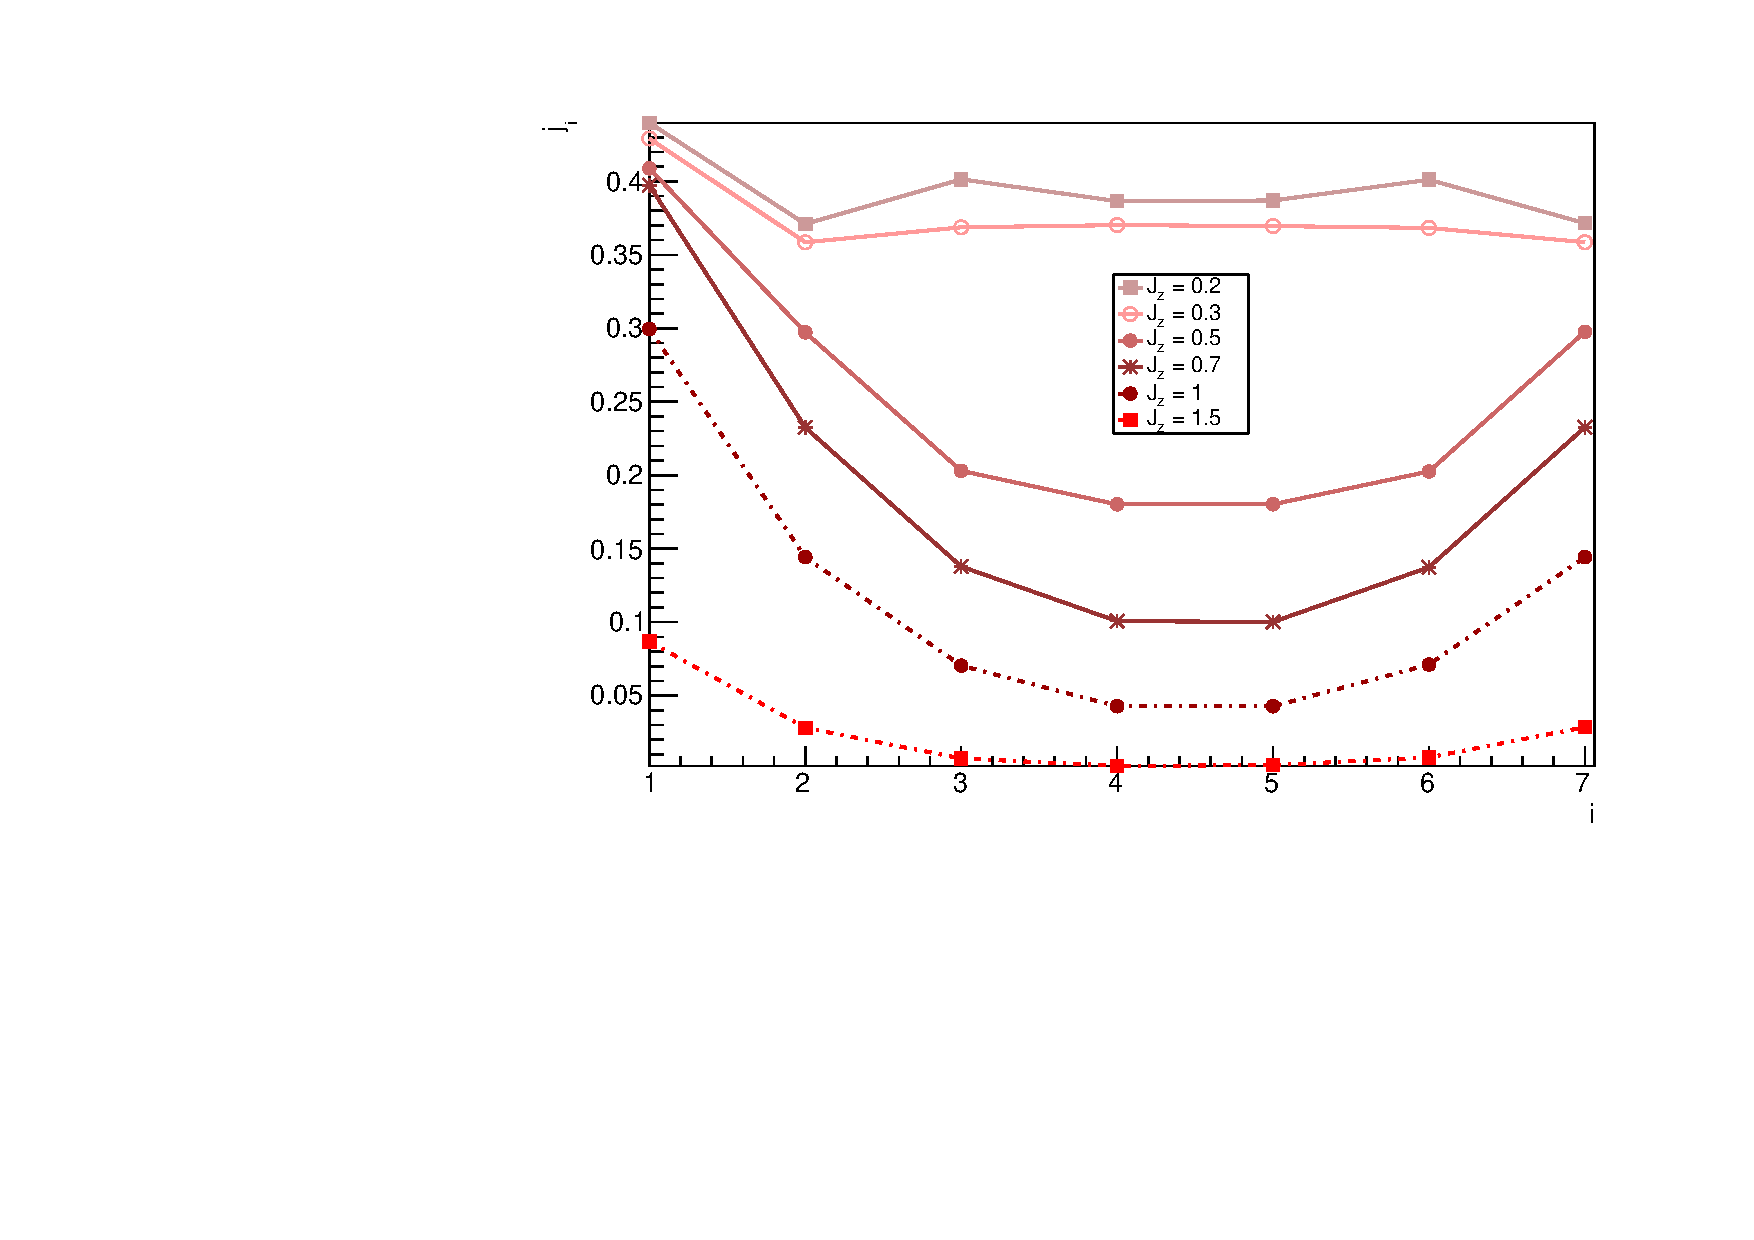
\includegraphics[scale=0.7]{Figures/8sites_spinCurrVSJz.pdf}
    %\caption{Spin current of a 8-sites chain, with $\gamma = 1$ for several values of $J_z$. Data %obtained from MPO method.}
    %\label{fig:8sites_spinCurrVSJz}
%\end{figure}

%\begin{figure}[H]
    %\centering
    %\includegraphics[scale=0.7]{Figures/8sites/8sites_spinCurrVSJz%QT.pdf}
    %\captionsetup{width=1.\linewidth}
    %\caption{Spin current of a 8-sites chain, with $\gamma = 1$ %for several values of $J_z$. Data obtained from QT method.}
    %\label{fig:8sites_spinCurrVSJzQT}
%\end{figure}

\begin{figure}[H]
    \centering
    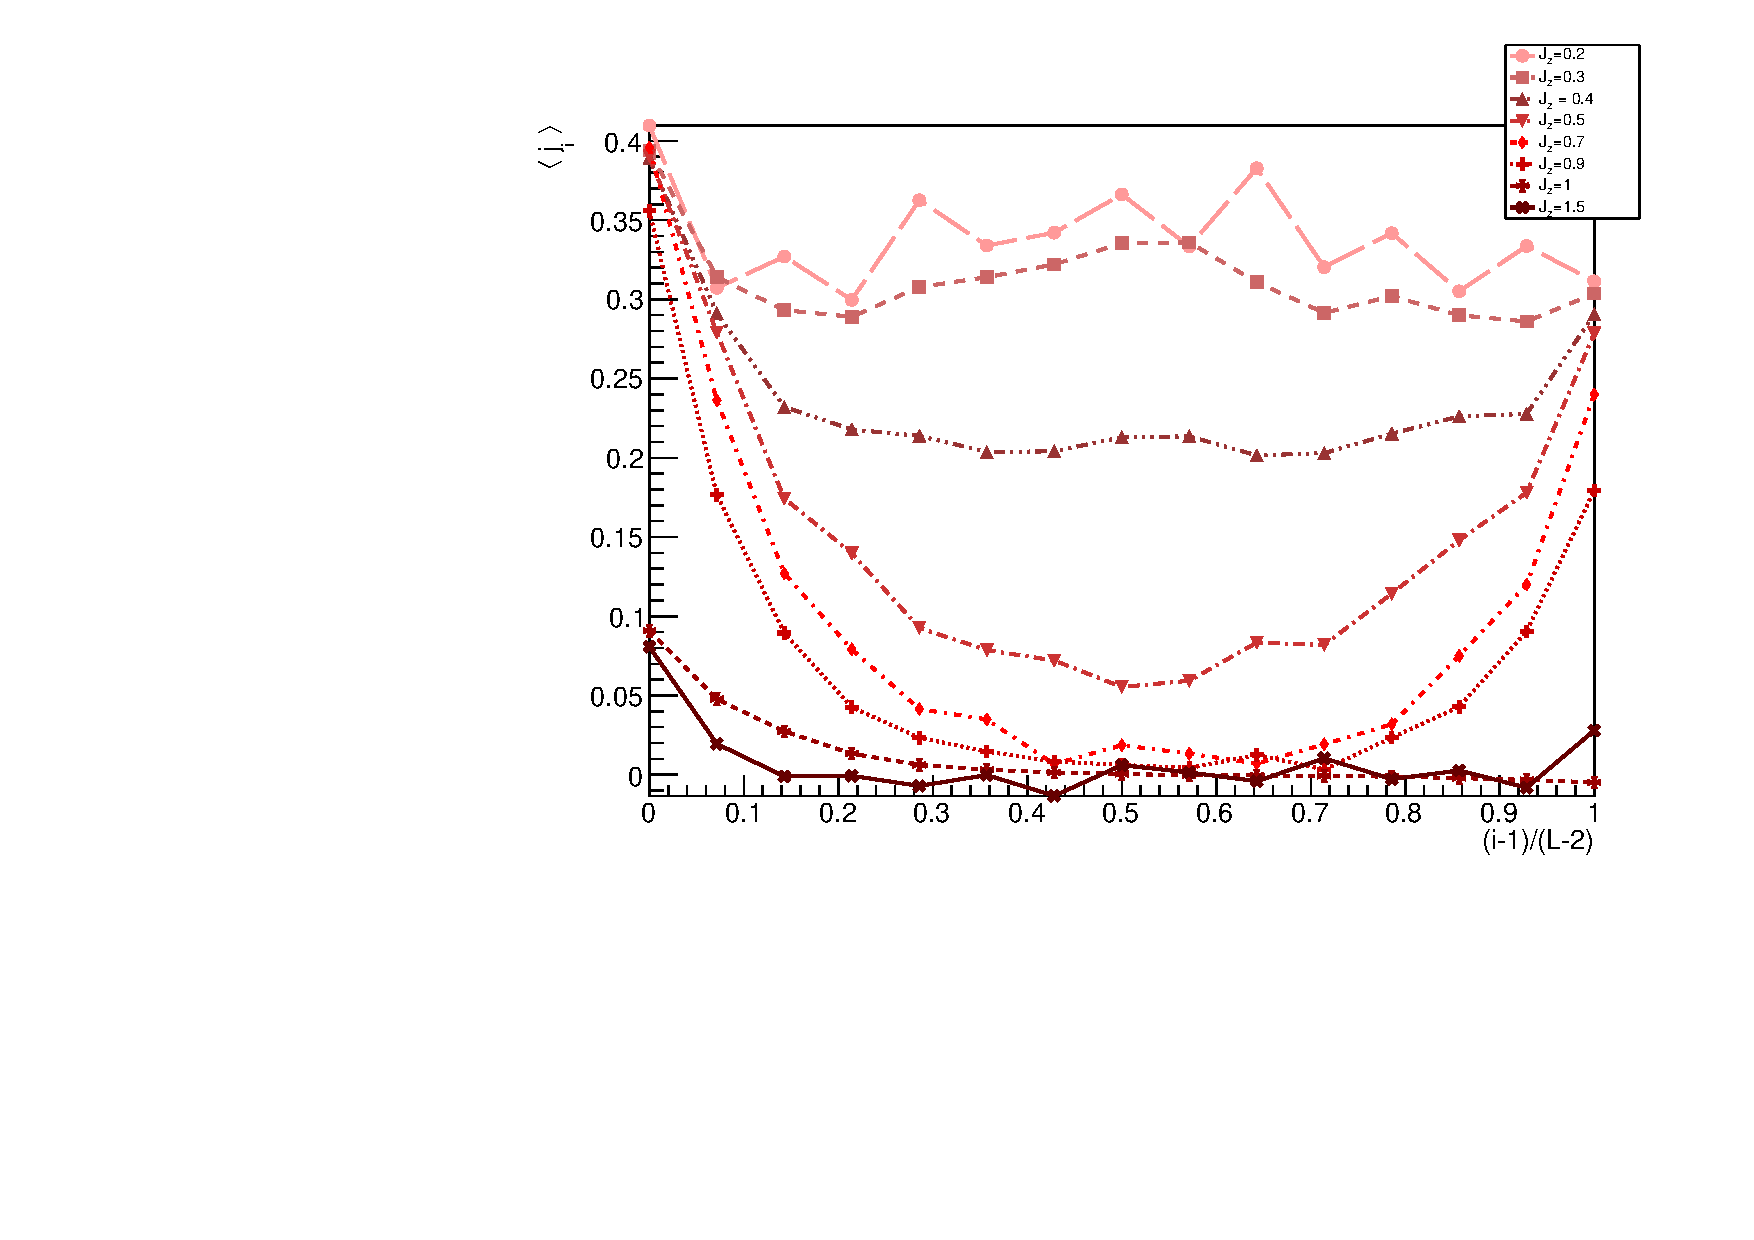
\includegraphics[scale=0.7]{Figures/16sites/16sites_SpinCurrVaryingJz.pdf}
    \captionsetup{width=1.\linewidth}
    \caption{Spin current of a 16-sites chain, with $\gamma = 1$ for several values of $J_z$. Data obtained from MPO method.}
    \label{fig:16sites_SpinCurrVaryingJz}
\end{figure}

The spin current between the first and the last two sites is independent from $J_z$, for $J_z < 1$; this can be a sign of the prevalence of dissipation over the Hamiltonian dynamics. Otherwise, for $J_z \geq 1$ the peak values (i.e. the spin current between the first two and the last two sites of the chain) drop while $J_z$ increases; this can be a sign of the growing prevalence of the Hamiltonian over the dissipation, while the coupling $J_z$ grows.

For the small values of $J_z$, i.e. for $J_z < 0.5$, the $\sigma_i^z\sigma_{i+1}^z$ term acts as a perturbation of the XY model. For this values, the spin current shows a discontinuous behaviour: the trend of spin current in the middle sites (i.e. all the sites excluding the first and the last) is almost constant. This is an additional sign of the prevalence of the role of dissipation.

For values of $J_z \geq 0.5$, the trend of the spin current is polynomial, with smooth decrease and increase nearby the ends of the chain; while $J_z$ grows, in the middle sites the spin current is more and more constant, sign of the fact that the role of Hamiltonian is more and more predominant. 

This irregular behaviour is suggestive of a phase transition; in order to get some numerical evidence of it, we have analyzed also the magnetization profile and the correlation function.

%\begin{figure}[H]
    %\centering
    %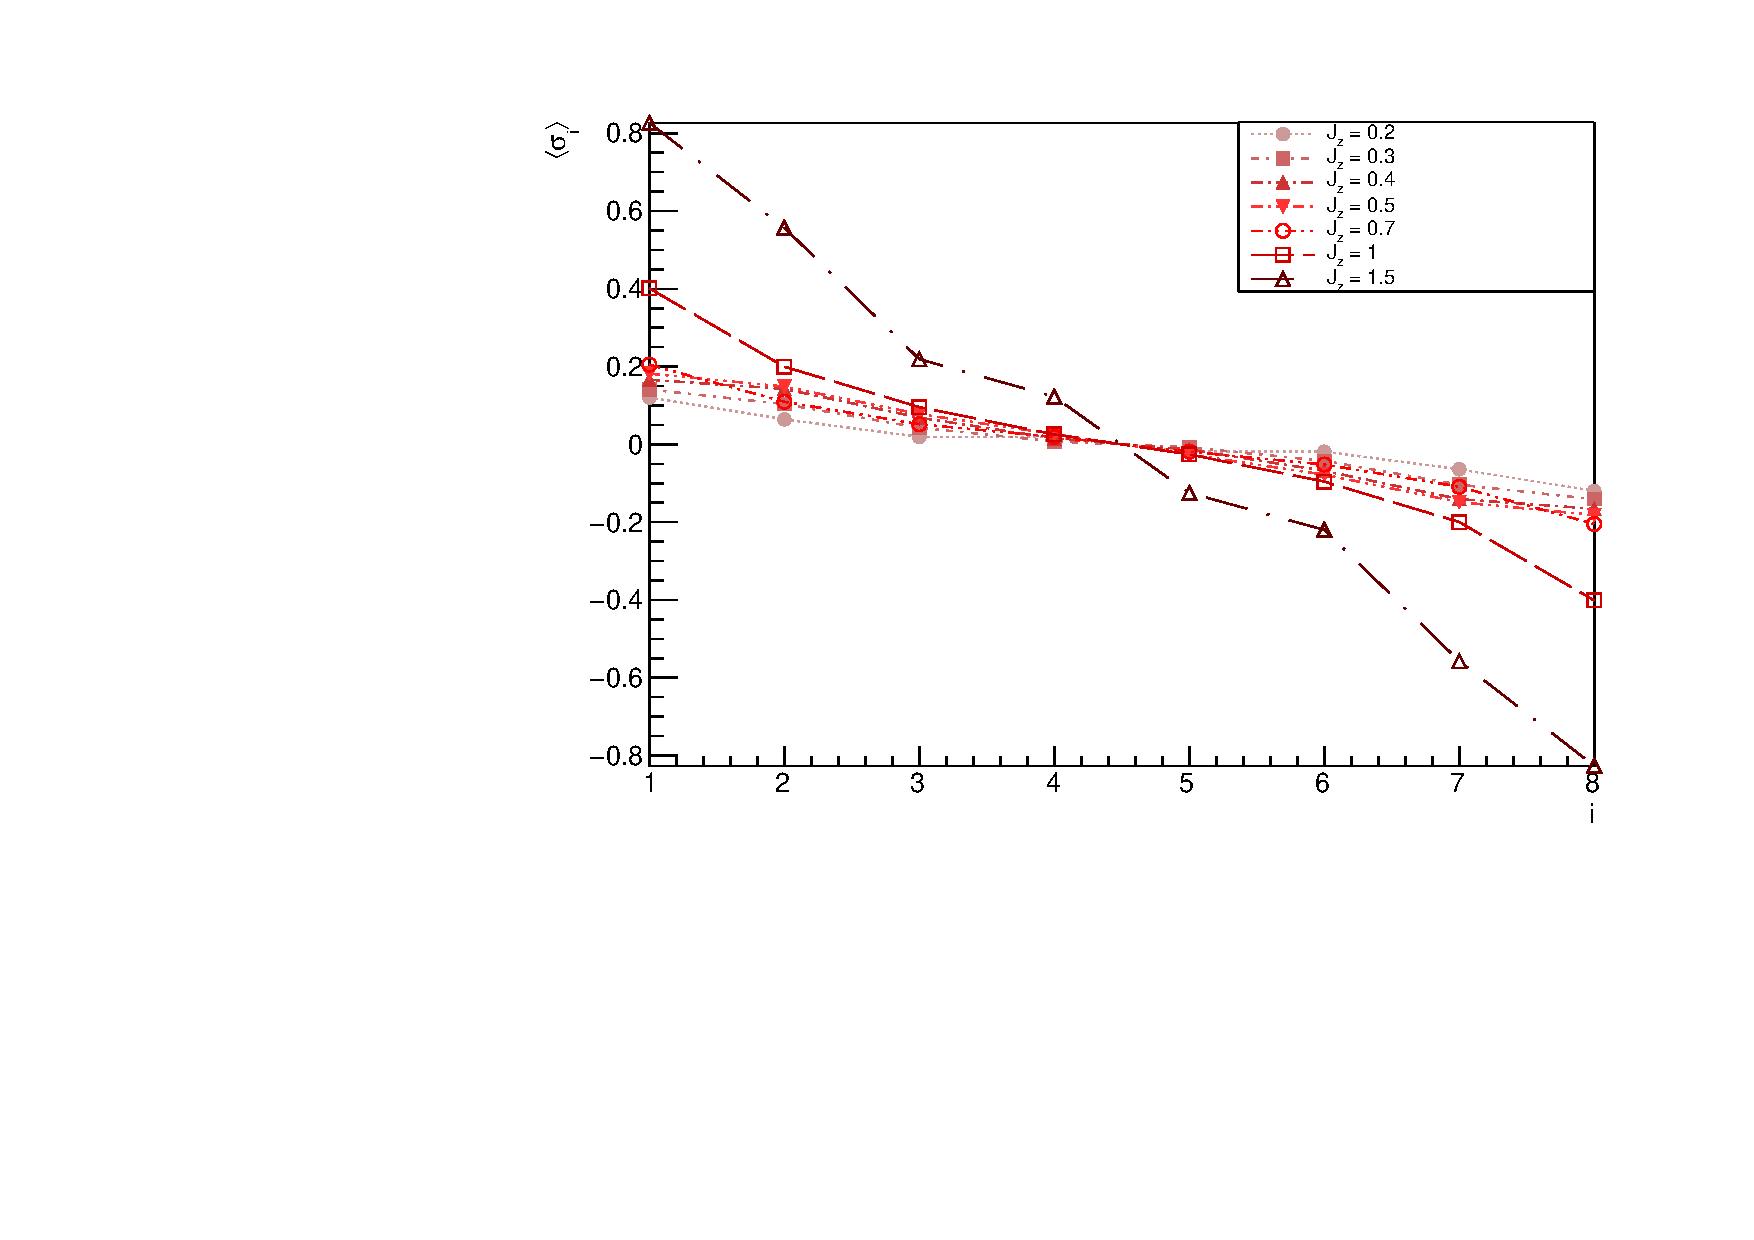
\includegraphics[scale=0.7]{Figures/8sites_LMvsJz.pdf}
    %\caption{Magnetization profile of a 8-sites chain, with $\gamma = 1$ for %several values of $J_z$. Data obtained from MPO method.}
    %\label{fig:8sites_LMvsJz}
%\end{figure}

%\begin{figure}[H]
    %\centering
    %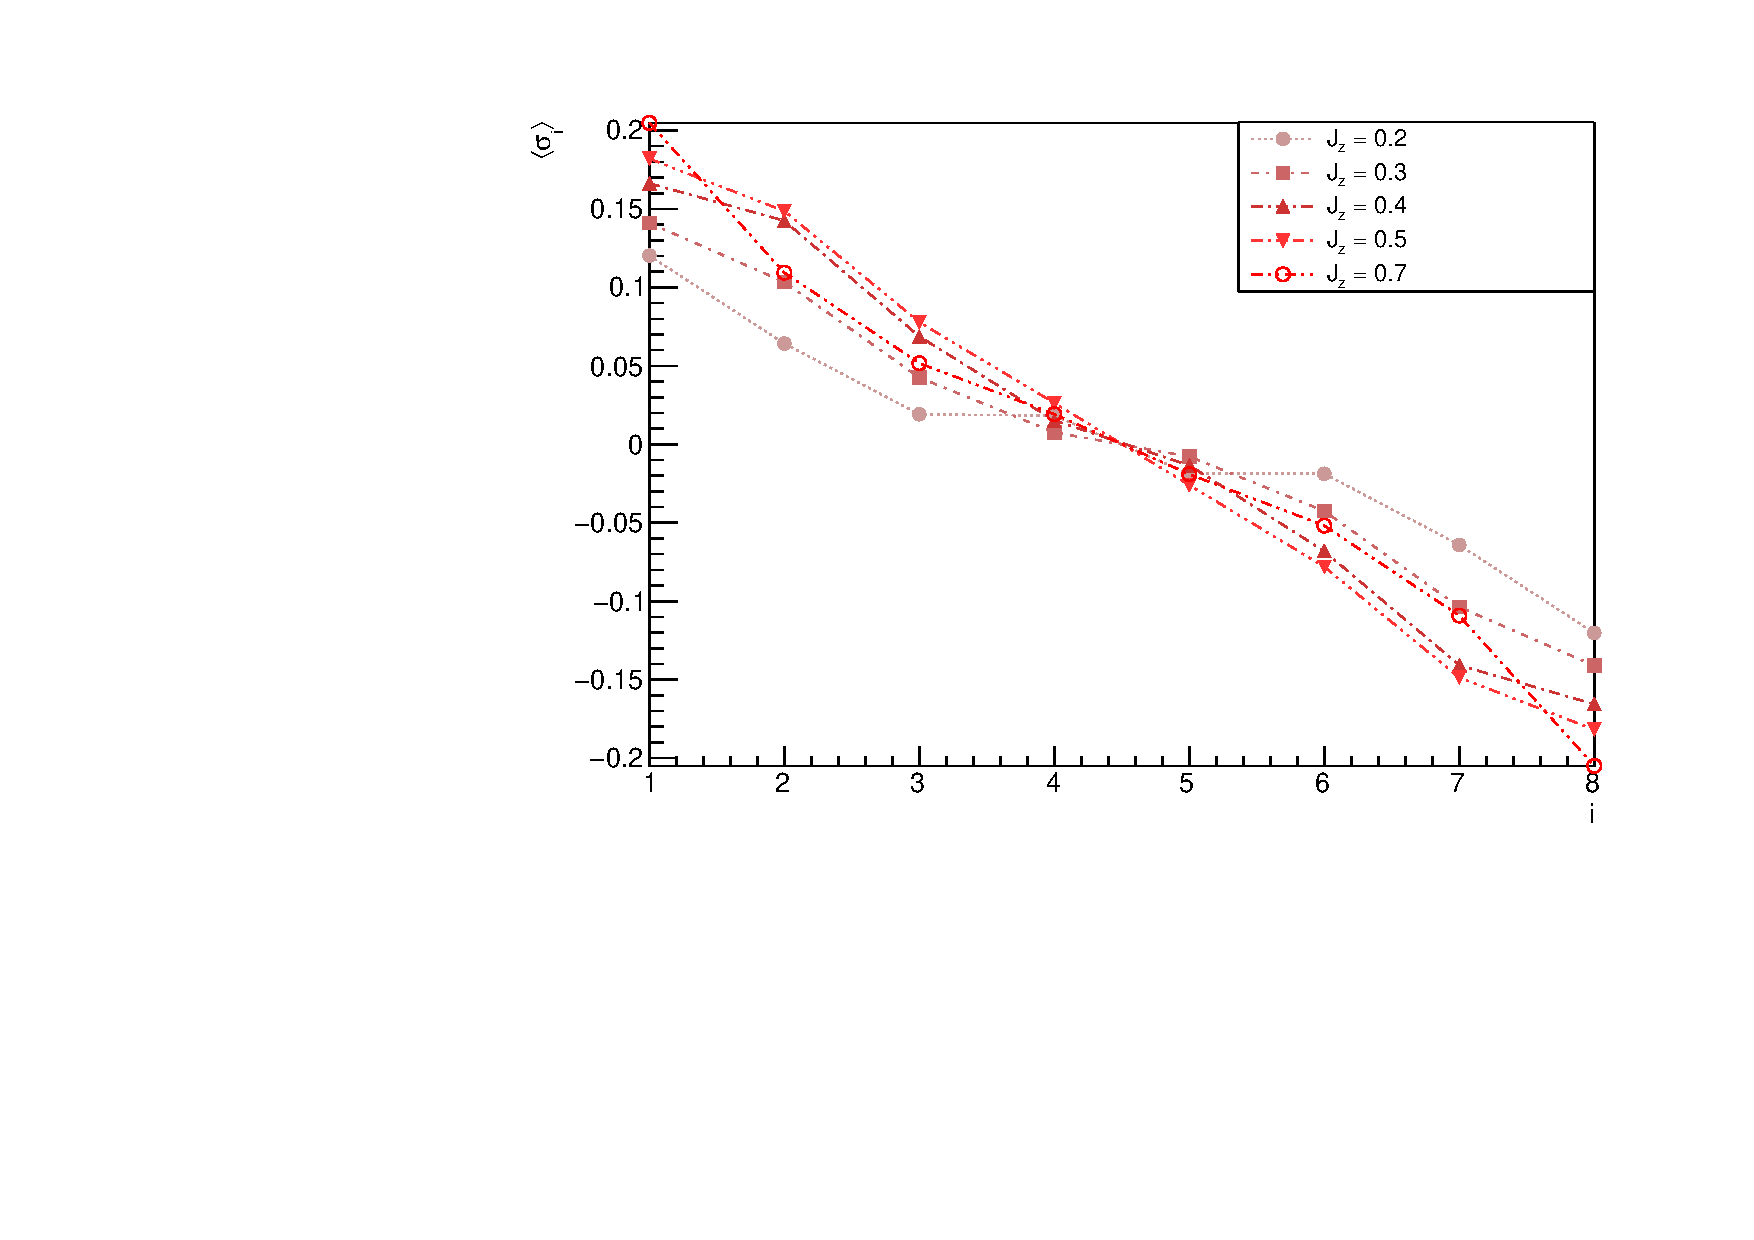
\includegraphics[scale=0.7]{Figures/8sites_LMvsLowJz.pdf}
    %\caption{Magnetization profile of a 8-sites chain, with $\gamma = 1$ for $J_z %\leq 0.7$. Data obtained from MPO method.}
    %\label{fig:8sites_LMvsLowJz}
%\end{figure}

%\begin{figure}[H]
    %\centering
    %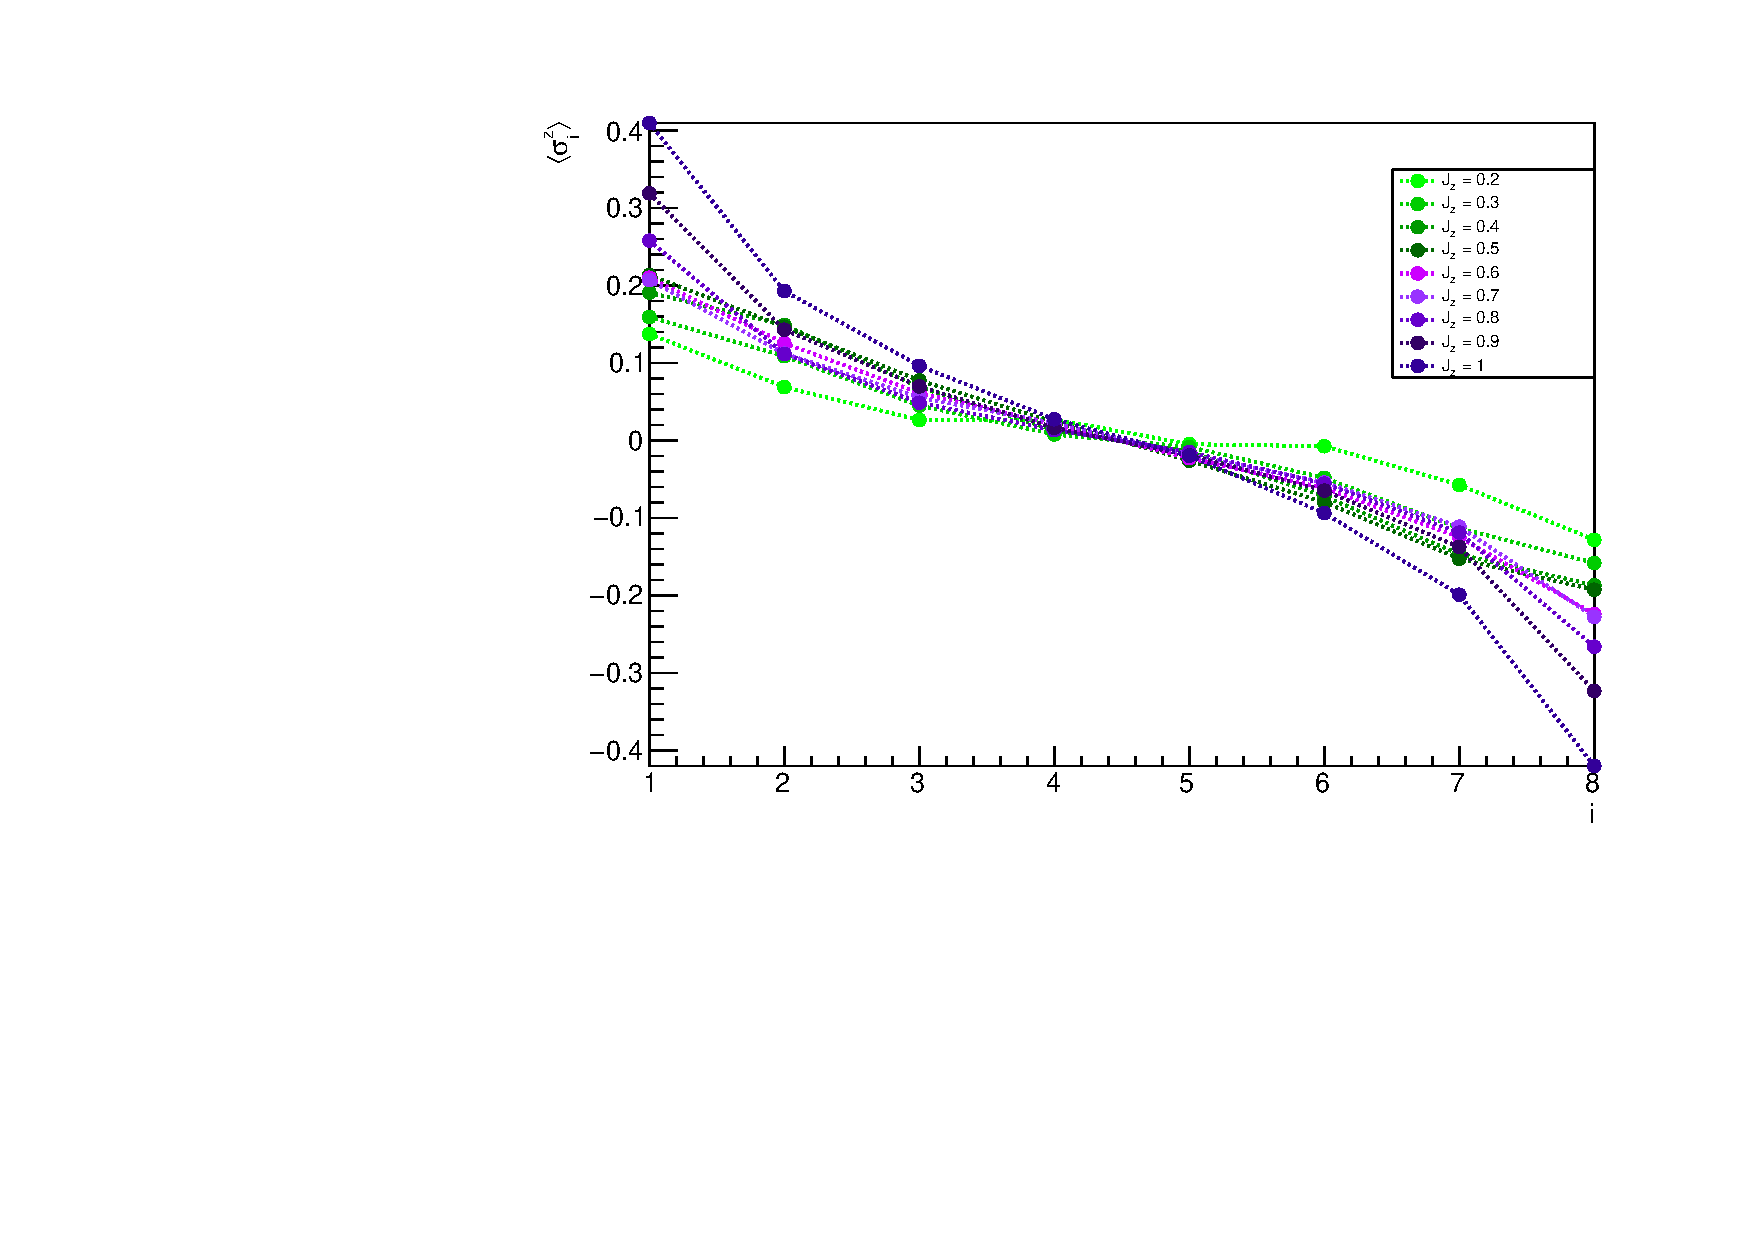
\includegraphics[scale=0.7]{Figures/8sites/8sites_LMvsJzQT.pdf}
    %\caption{Magnetization profile of a 8-sites chain, with $\gamma = 1$ for %several values of $J_z$. Data obtained from QT method.}
    %\label{fig:8sites_LMvsJzQT}
%\end{figure}

%\begin{figure}[H]
    %\centering
    %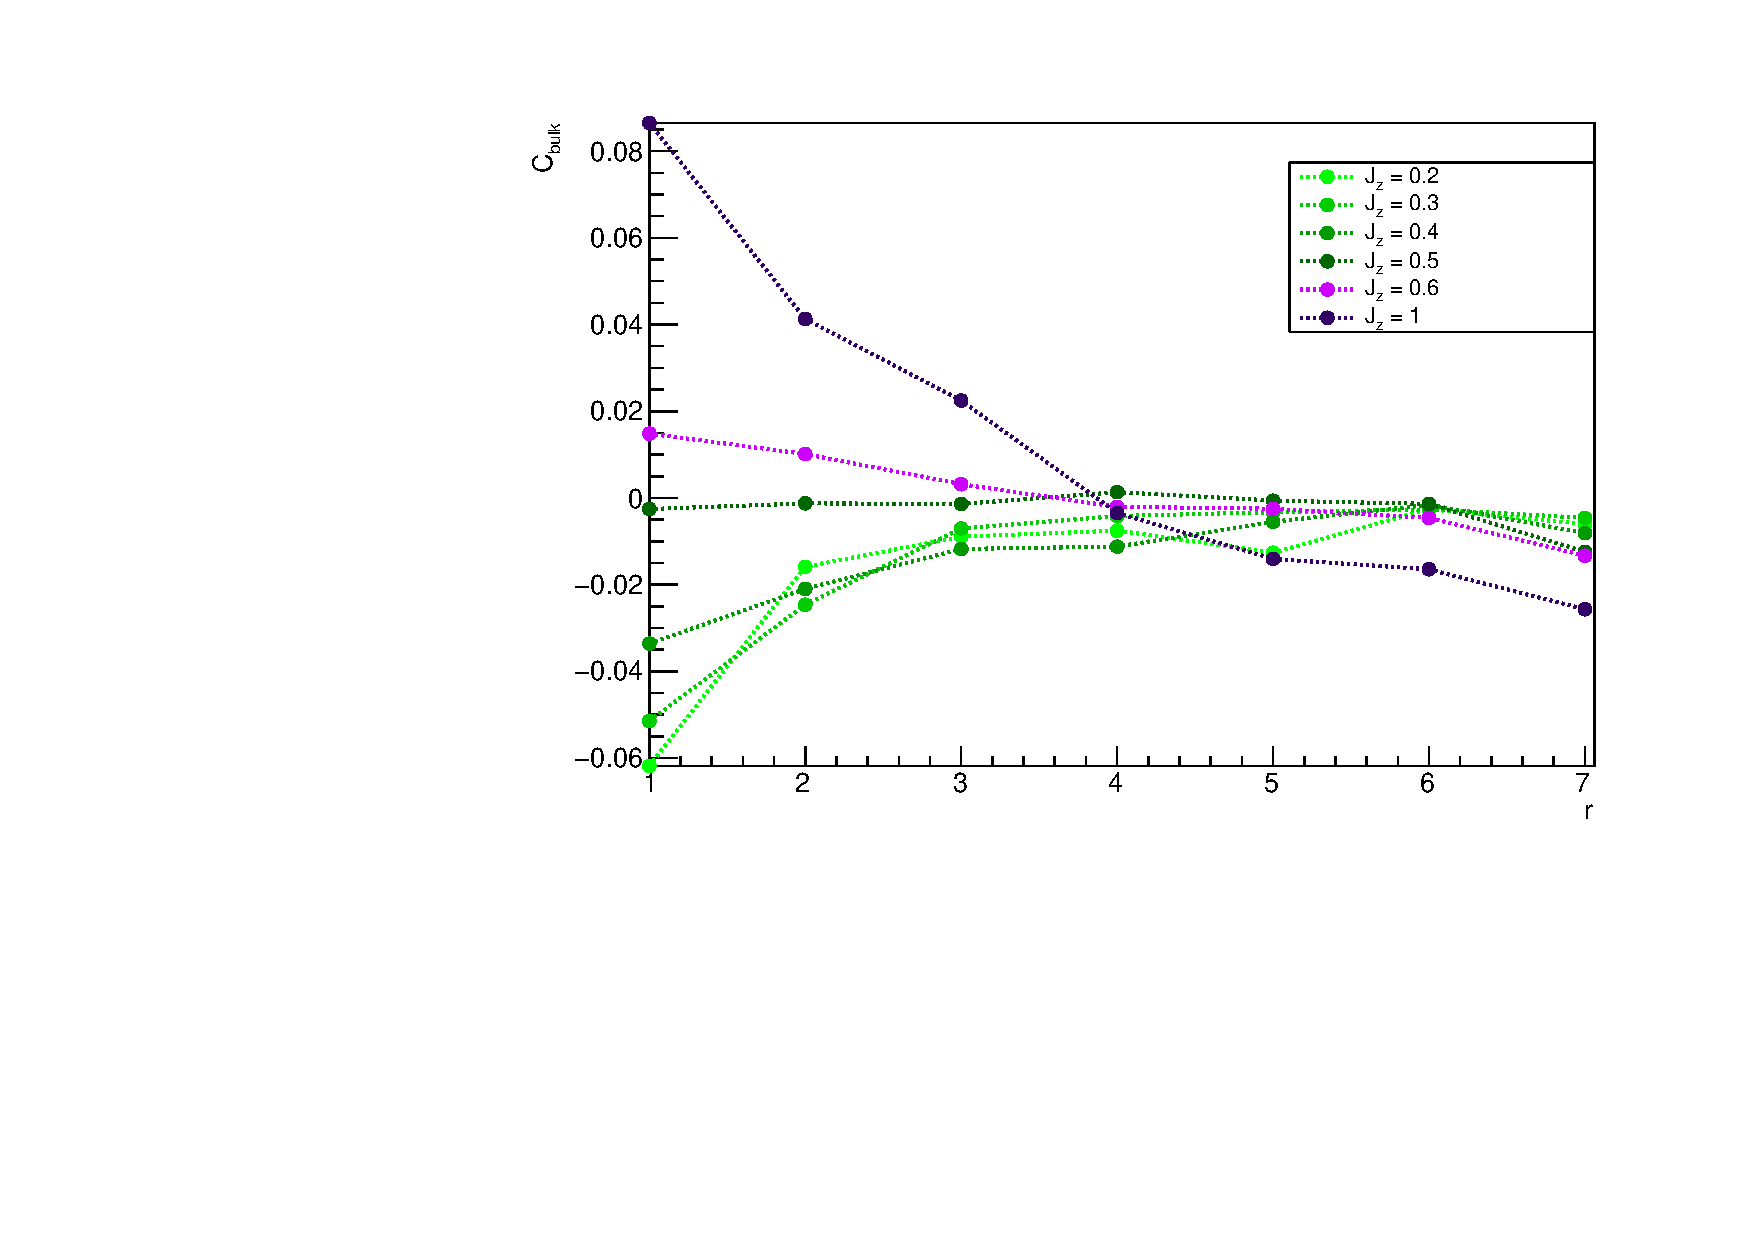
\includegraphics[scale=0.7]{Figures/8sites/8sites_CFBulkvsLowJz_QT.pdf}
    %\caption{Bulk correlation function of a 8-sites chain, with $\gamma = 1$ for %several values of $J_z \leq 1$. Data obtained from QT method.}
    %\label{fig:8sites_CFBulkvsLowJz_QT}
%\end{figure}


%\begin{figure}[H]
    %\centering
    %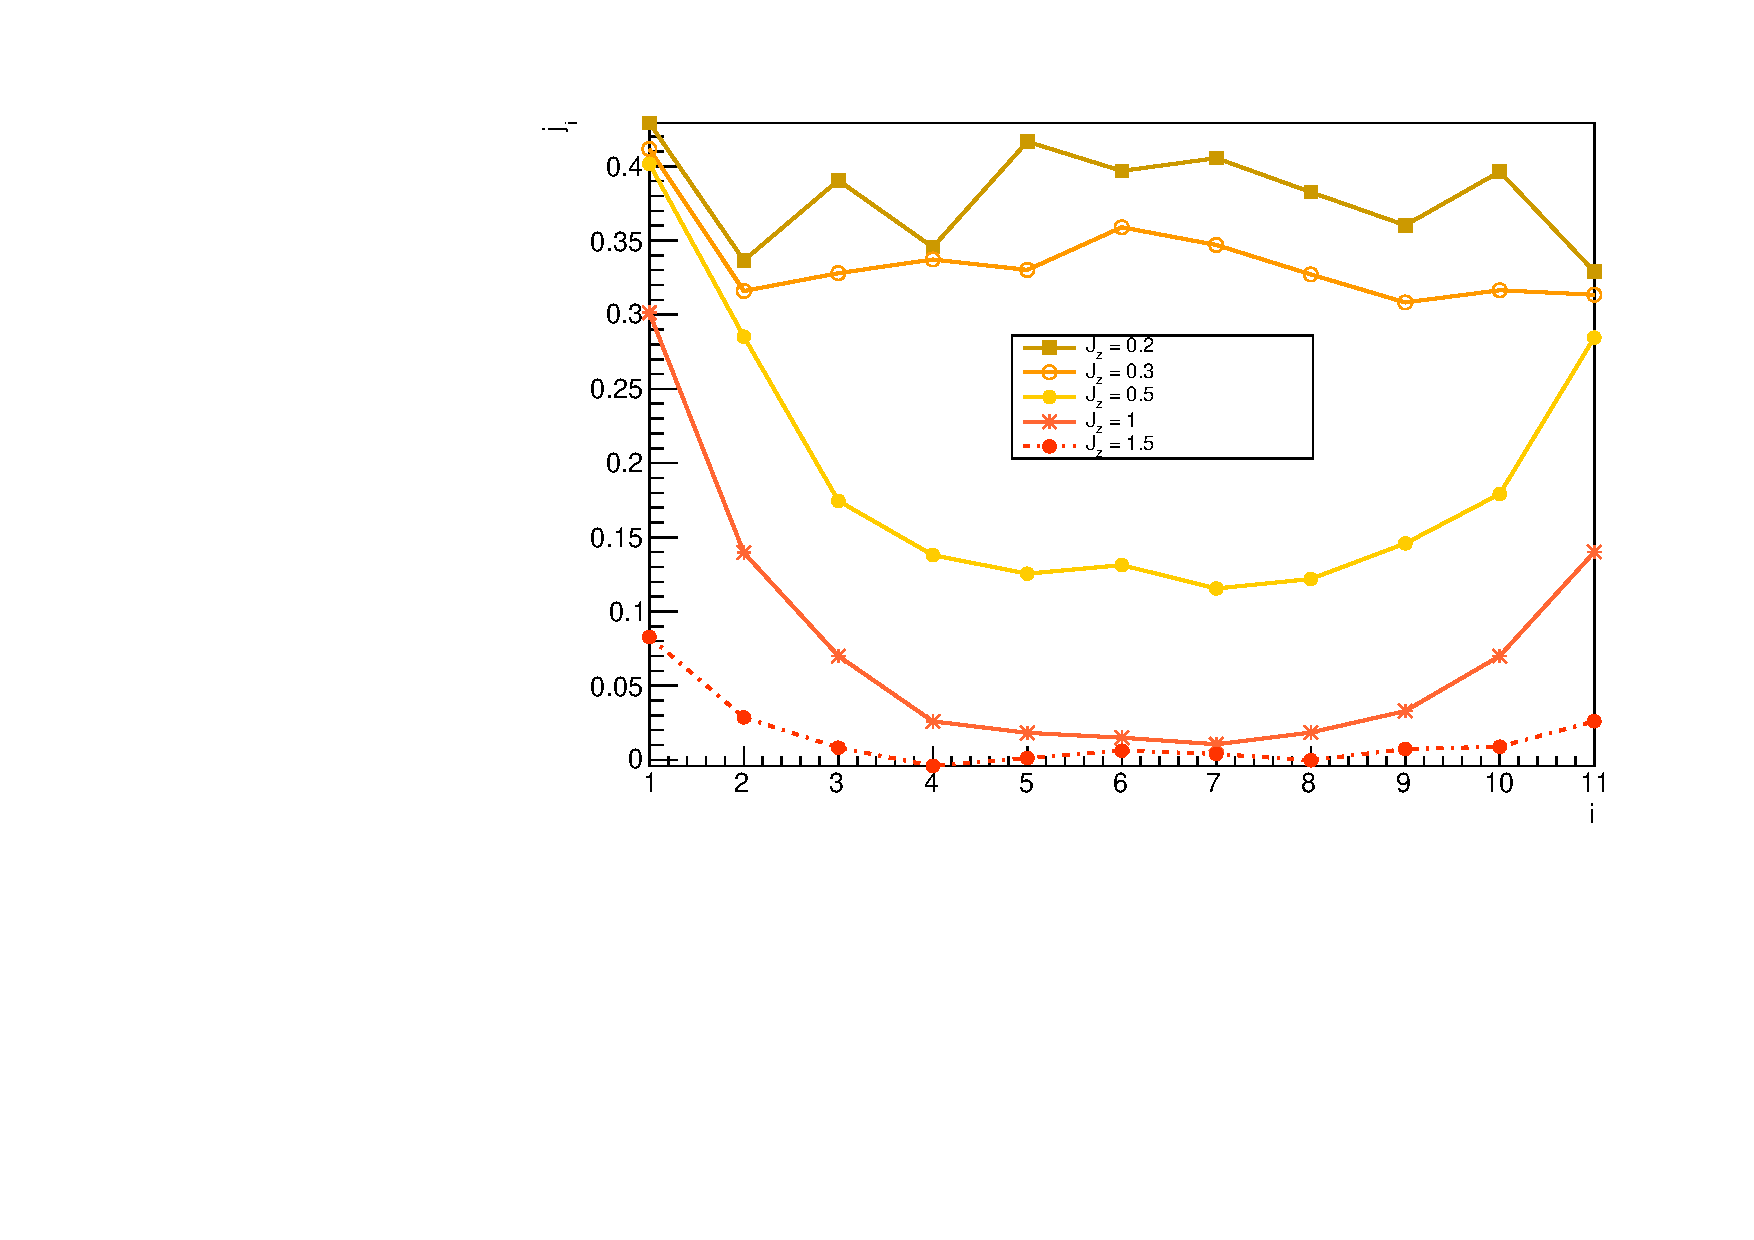
\includegraphics[scale=0.7]{Figures/12sites_spinCurrVSJz.pdf}
    %\caption{Spin current of a 12-sites chain, with $\gamma = 1$ for several values %of $J_z$. Data obtained from MPO method.}
    %\label{fig:12sites_spinCurrVSJz}
%\end{figure}

%\begin{figure}[H]
    %\centering
    %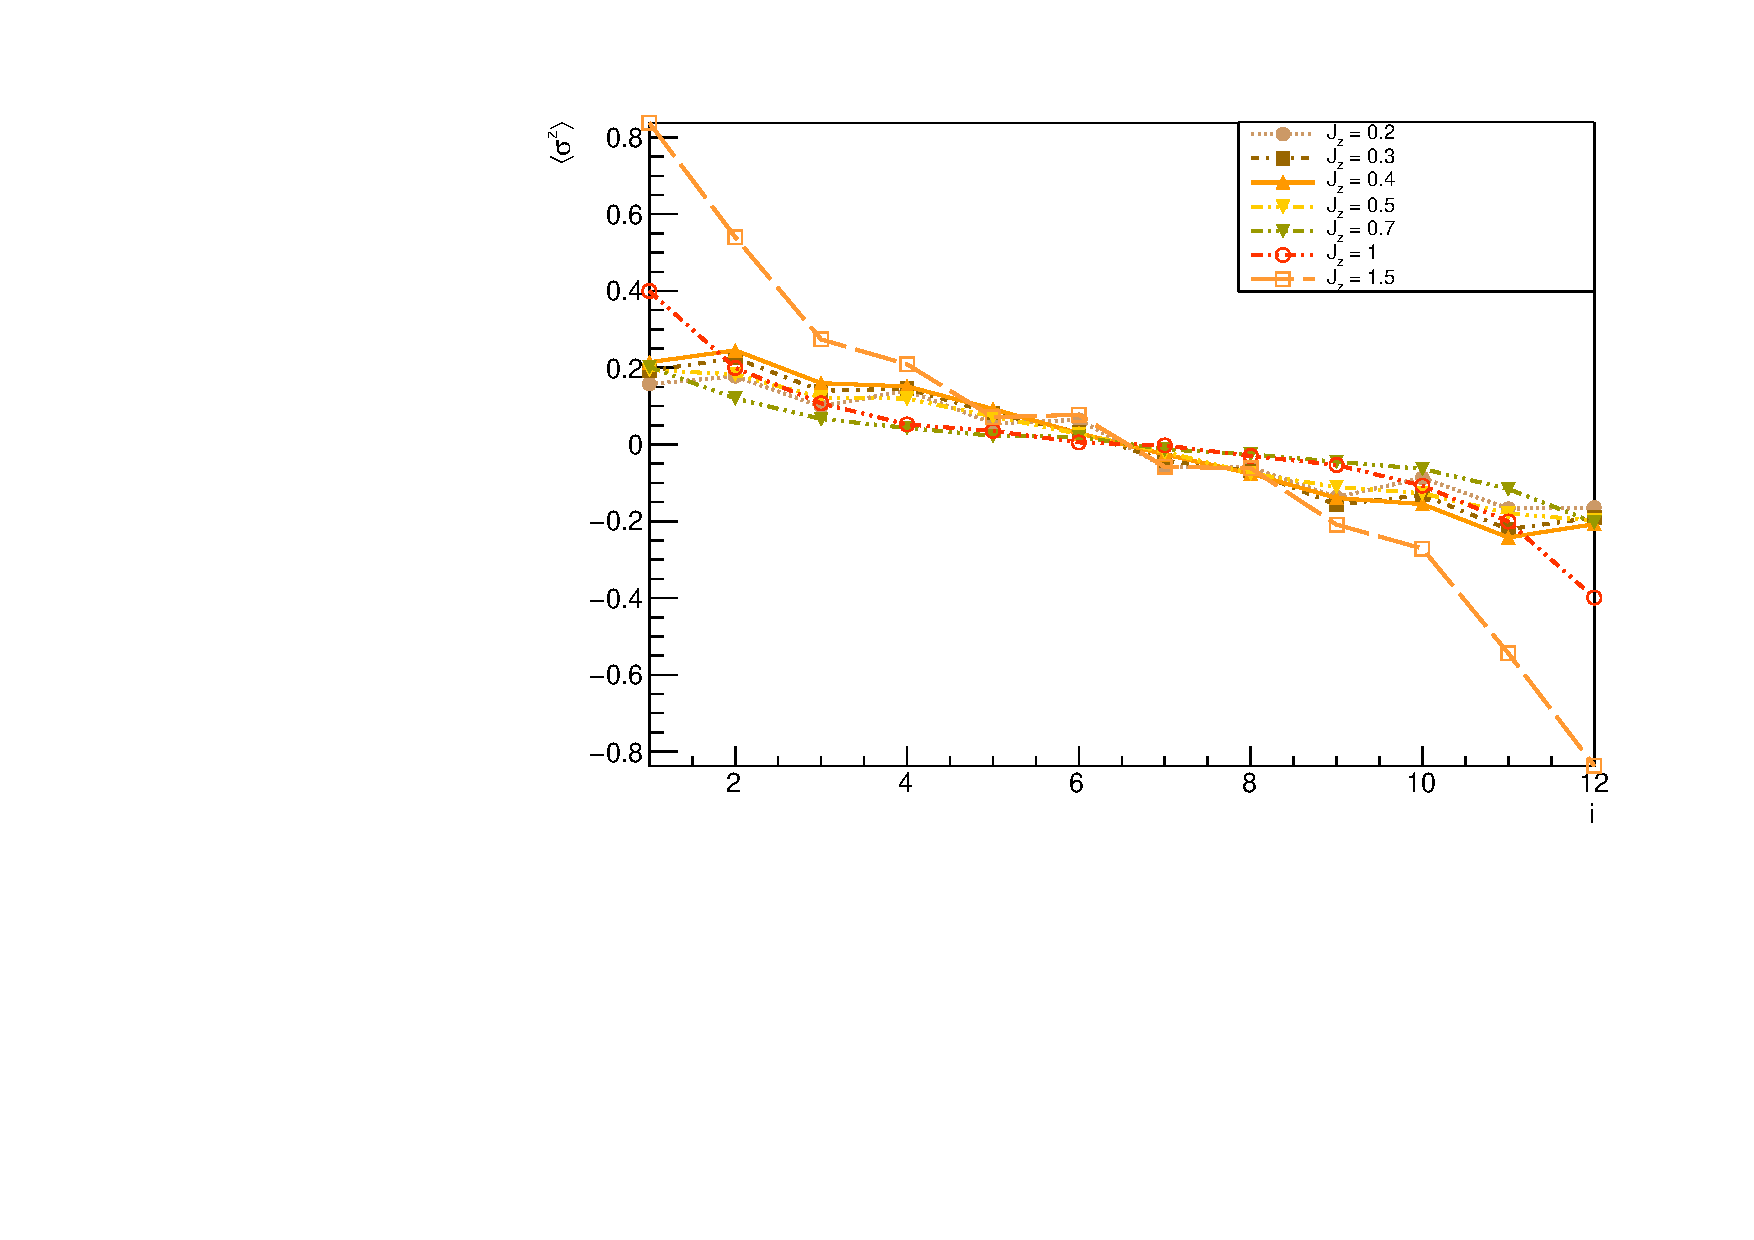
\includegraphics[scale=0.7]{Figures/12sites/12sites_LMvsJz.pdf}
    %\caption{Magnetization profile of a 12-sites chain, with $\gamma = 1$ for $J_z %\leq 0.7$. Data obtained from MPO method.}
    %\label{fig:my_label}
%\end{figure}

%\begin{figure}[H]
    %\centering
    %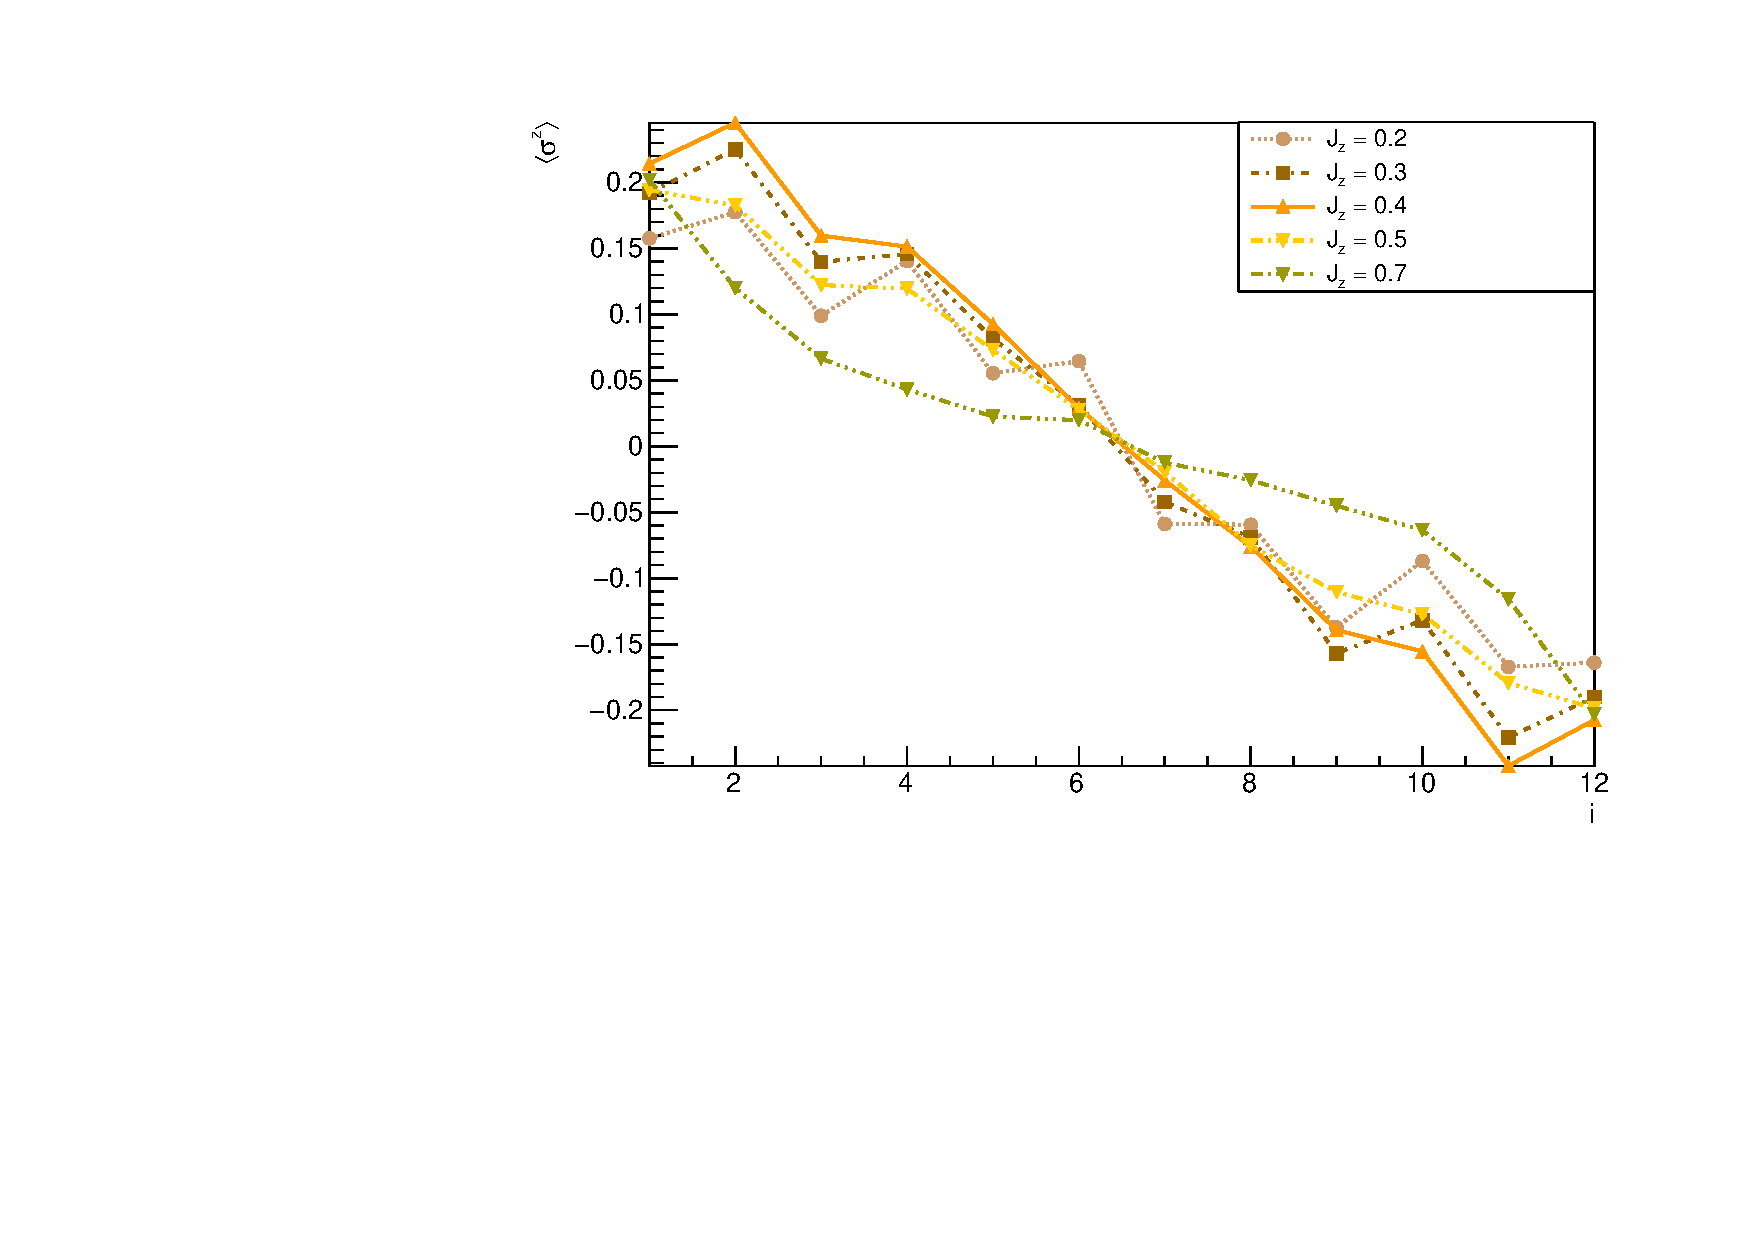
\includegraphics[scale=0.7]{Figures/12sites/12sites_LMvsLOWJz.pdf}
    %\caption{Magnetization profile of a 12-sites chain, with $\gamma = 1$ for $J_z %\leq 0.7$. Data obtained from MPO method.}
    %\label{fig:my_label}
%\end{figure}

%\begin{figure}[H]
    %\centering
    %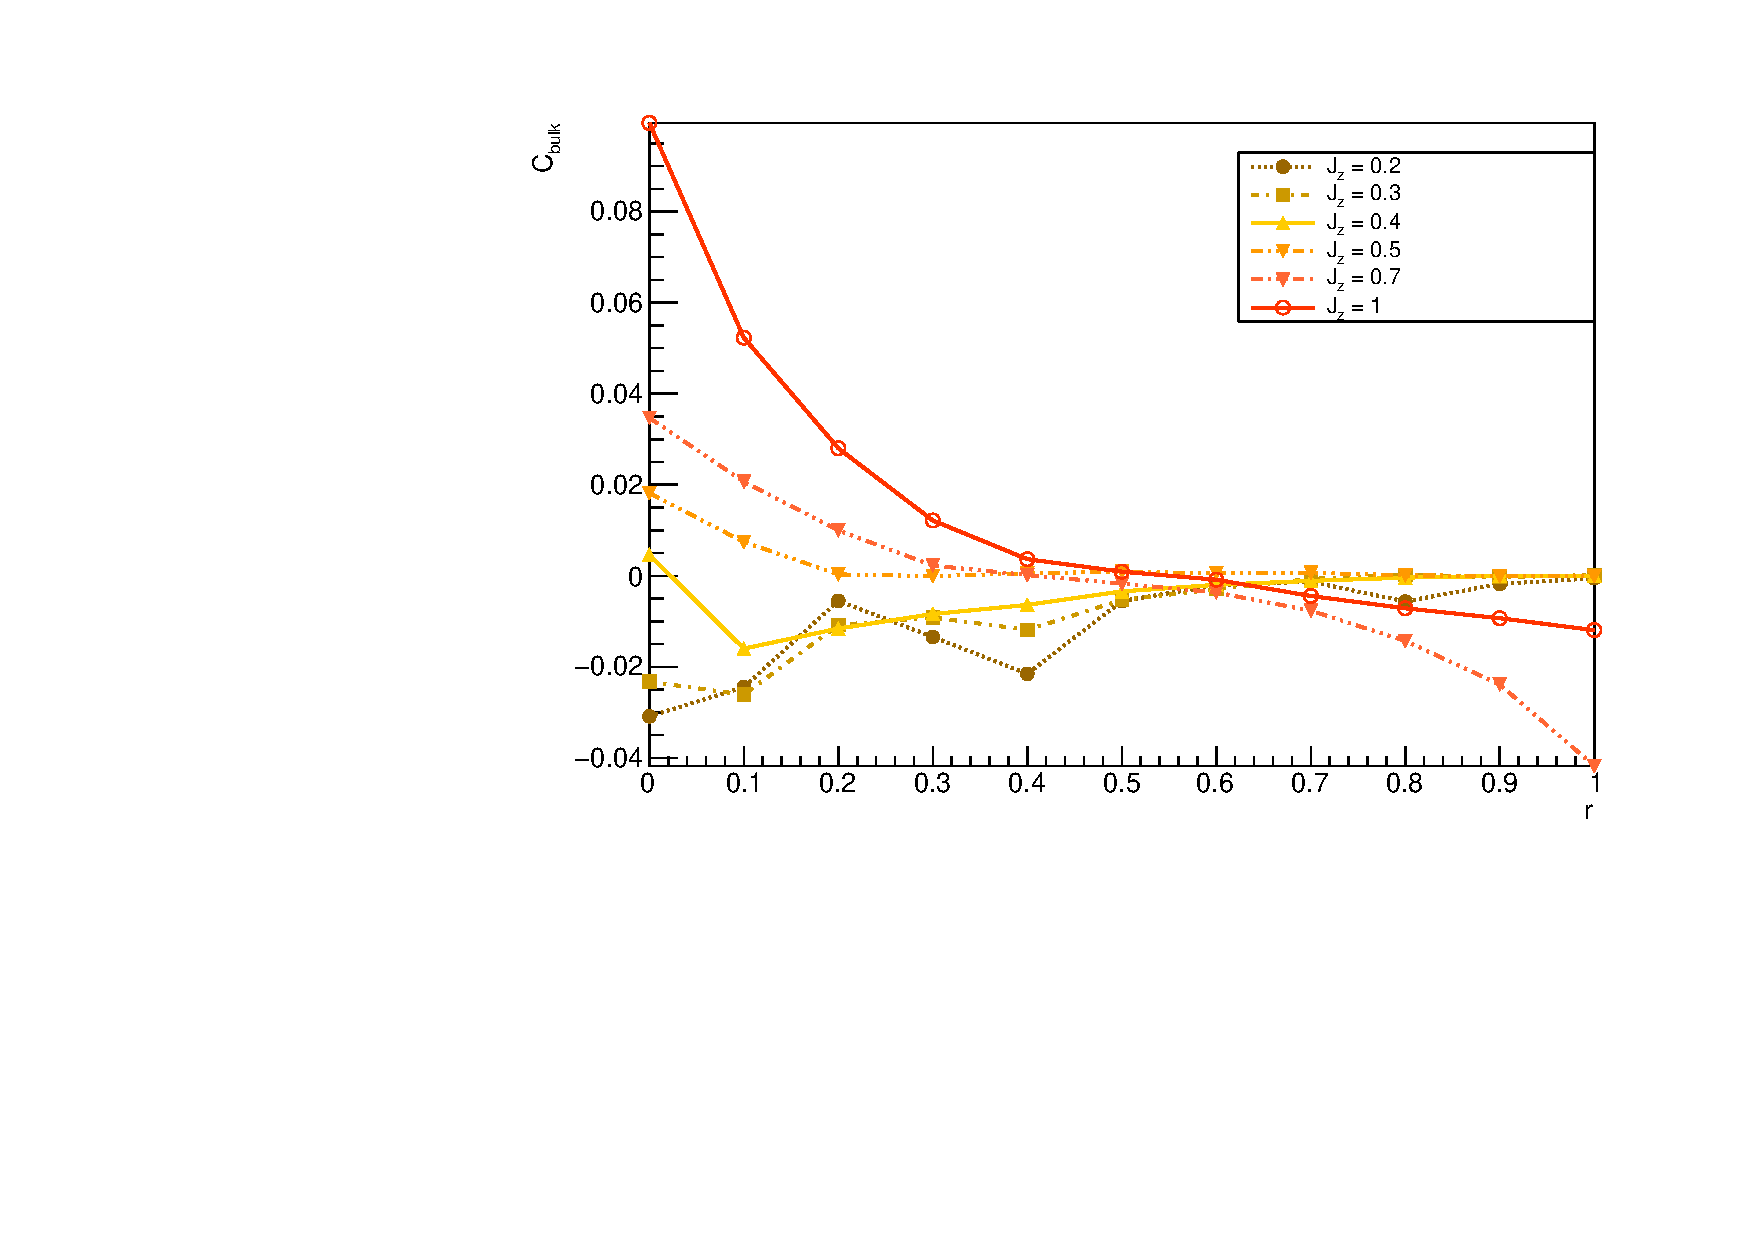
\includegraphics[scale=0.7]{Figures/12sites/12sites_CFBulkVSLowJz.pdf}
    %\caption{Bulk correlation function of a 12-sites chain, with $\gamma = 1$ for %several values of $J_z \leq 1$. Data obtained from MPO method.}
    %\label{fig:12sites_CFBulkVSLowJz}
%\end{figure}

\begin{figure}[H]
    \centering
    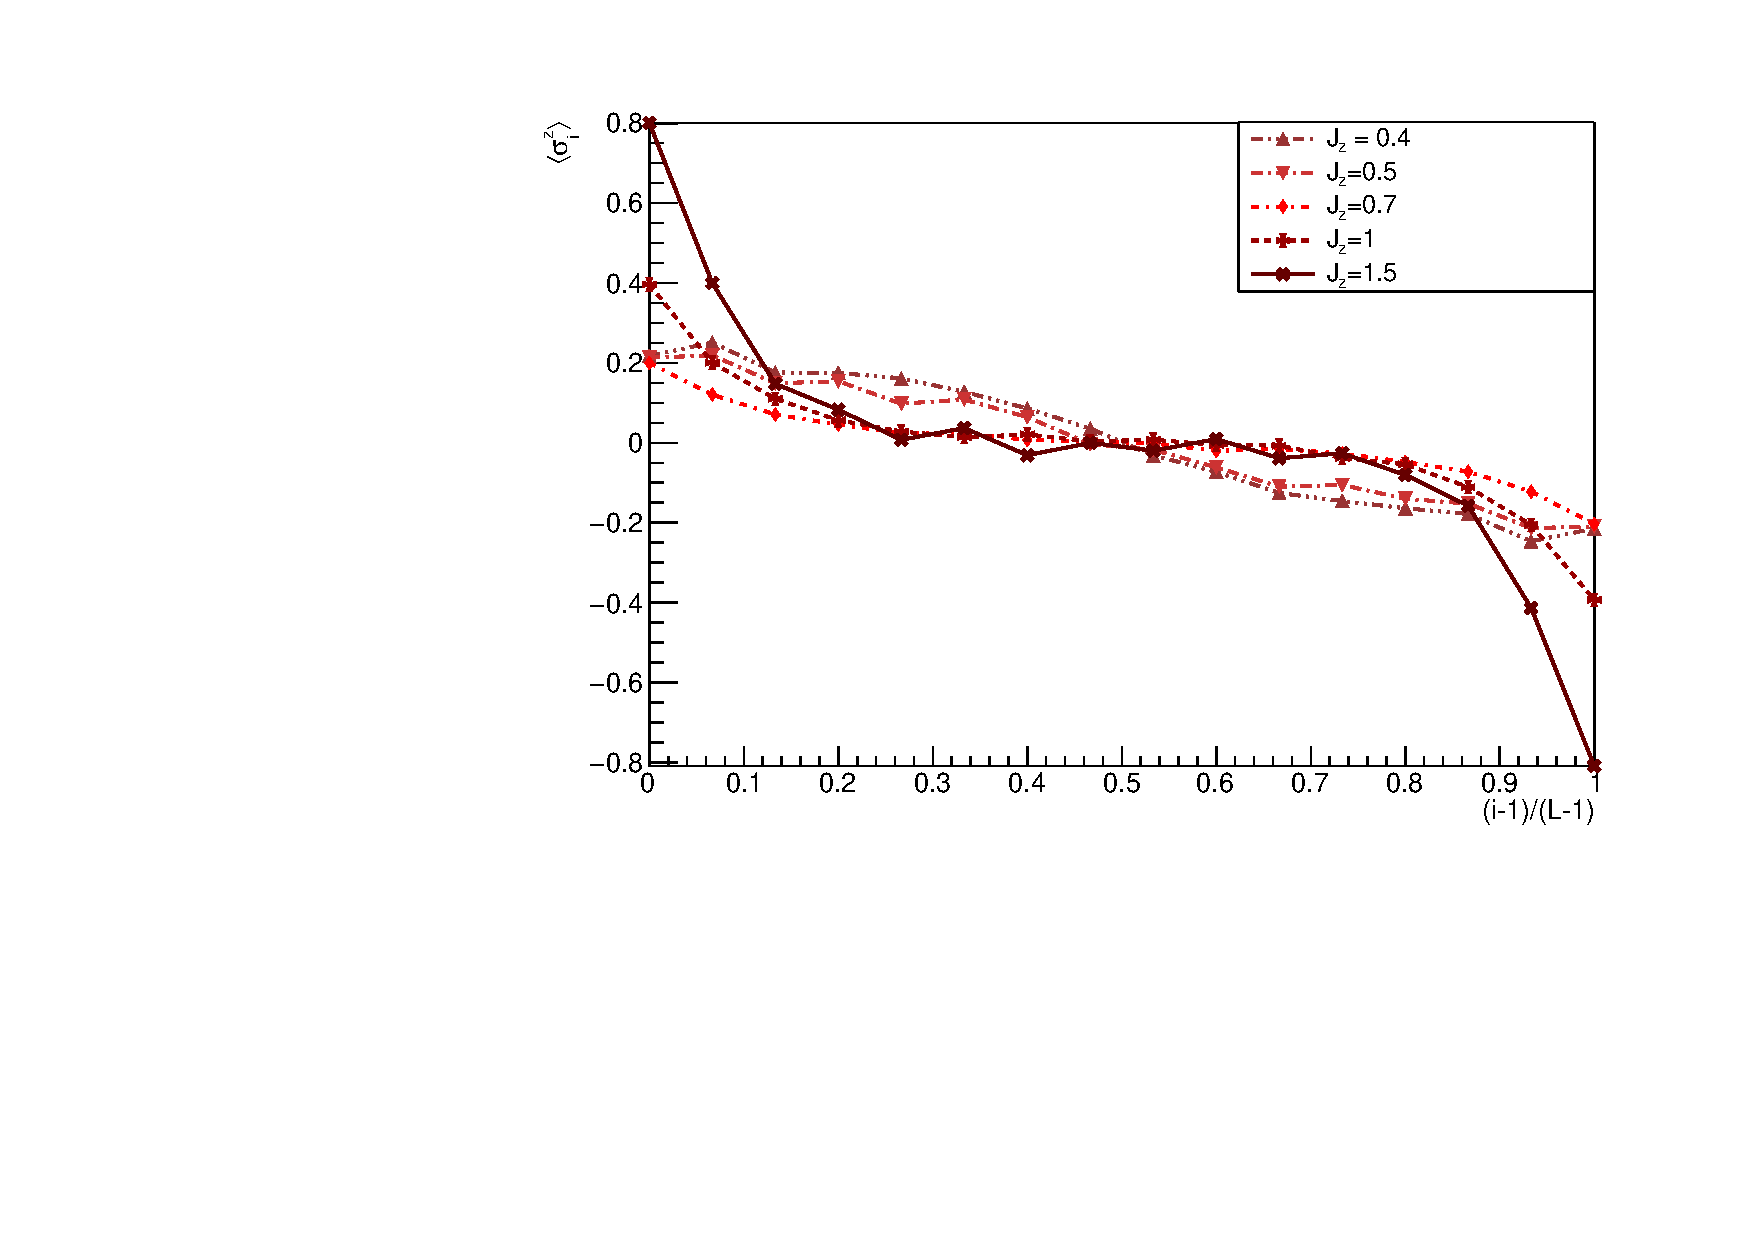
\includegraphics[scale=0.7]{Figures/16sites/16sites_LMvsJz.pdf}
    \captionsetup{width=1.\linewidth}
    \caption{Magnetization profile of a 16-sites chain, with $\gamma = 1$ for several values of $J_z$. Data obtained from MPO method.}
    \label{fig:16sites_LMvsJz}
\end{figure}

The magnetization profile (displayed in fig.~\ref{fig:16sites_LMvsJz}) for $J_z \geq 1$ shows a similar behaviour to the one seen in the previous chapter, when we considered variation of $\gamma$: the variation of the coupling constant $J_z$ has a similar effect of the one caused by the variation of the dissipation rate $\gamma$. 

For small values of $J_z$, i.e. $J_z < 1$, a couple of things can be noted. First of all, for all the $J_z < 1$ the $\langle \sigma^z \rangle$ of the first and of the last spin of the chain is constant. This can be explained as an unimportance of the Hamiltonian terms in relation to dissipation. 

It is worth noting that in the magnetization profile does not arise the discontinuity noticed in the trend of the spin current, for $J_z < 0.5$. Analyzing the two-point correlation function can be helpful in order to brighten this hypothesis.

%\begin{figure}[H]
    %\centering
    %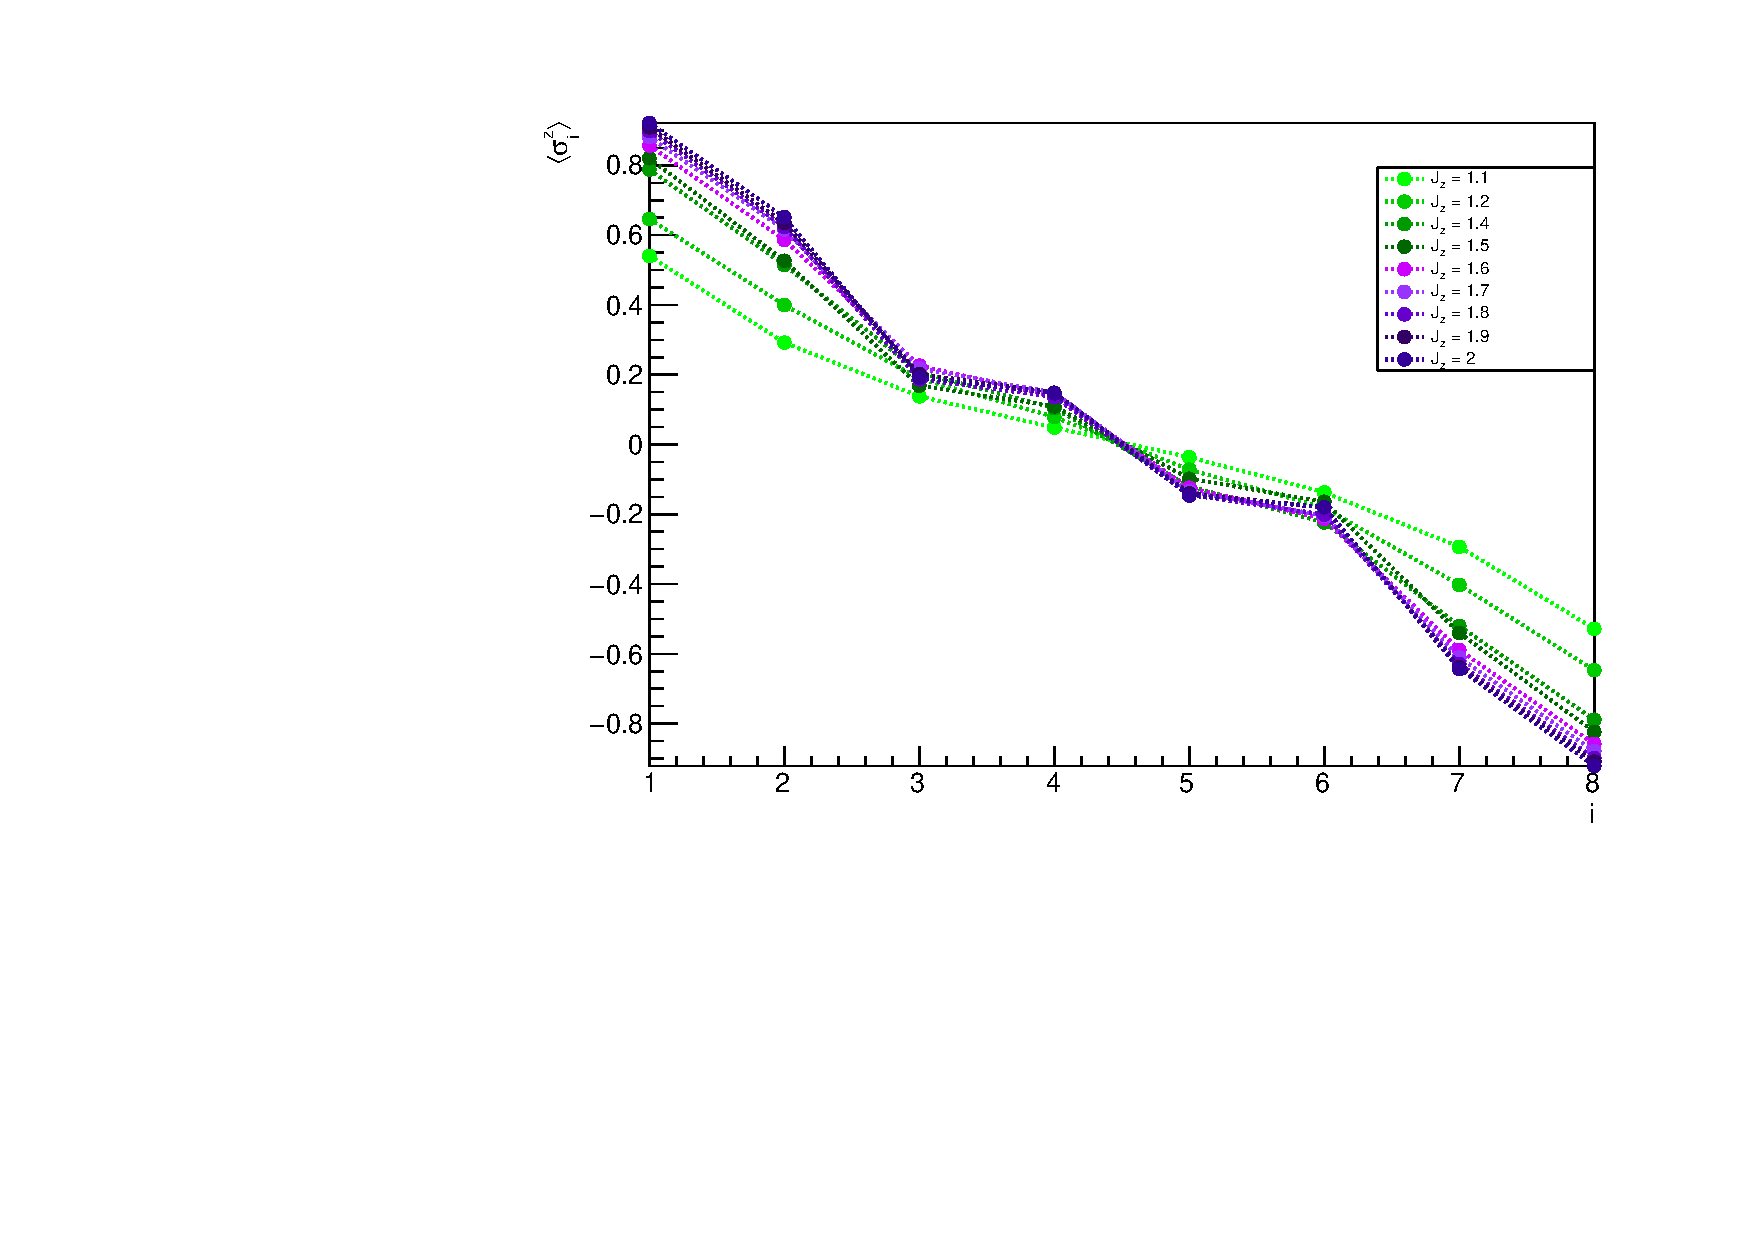
\includegraphics[scale=0.7]{Figures/8sites/8sites_LMvsJz_gtOneQT.pdf}
    %\caption{Magnetization profile of a 8-sites chain, with $\gamma = 1$ for %several values of $J_z \geq 1.1$. Data obtained from QT method.}
    %\label{fig:8sites_LMvsJz_gtOneQT}
%\end{figure}



\begin{figure}[H]
    \centering
    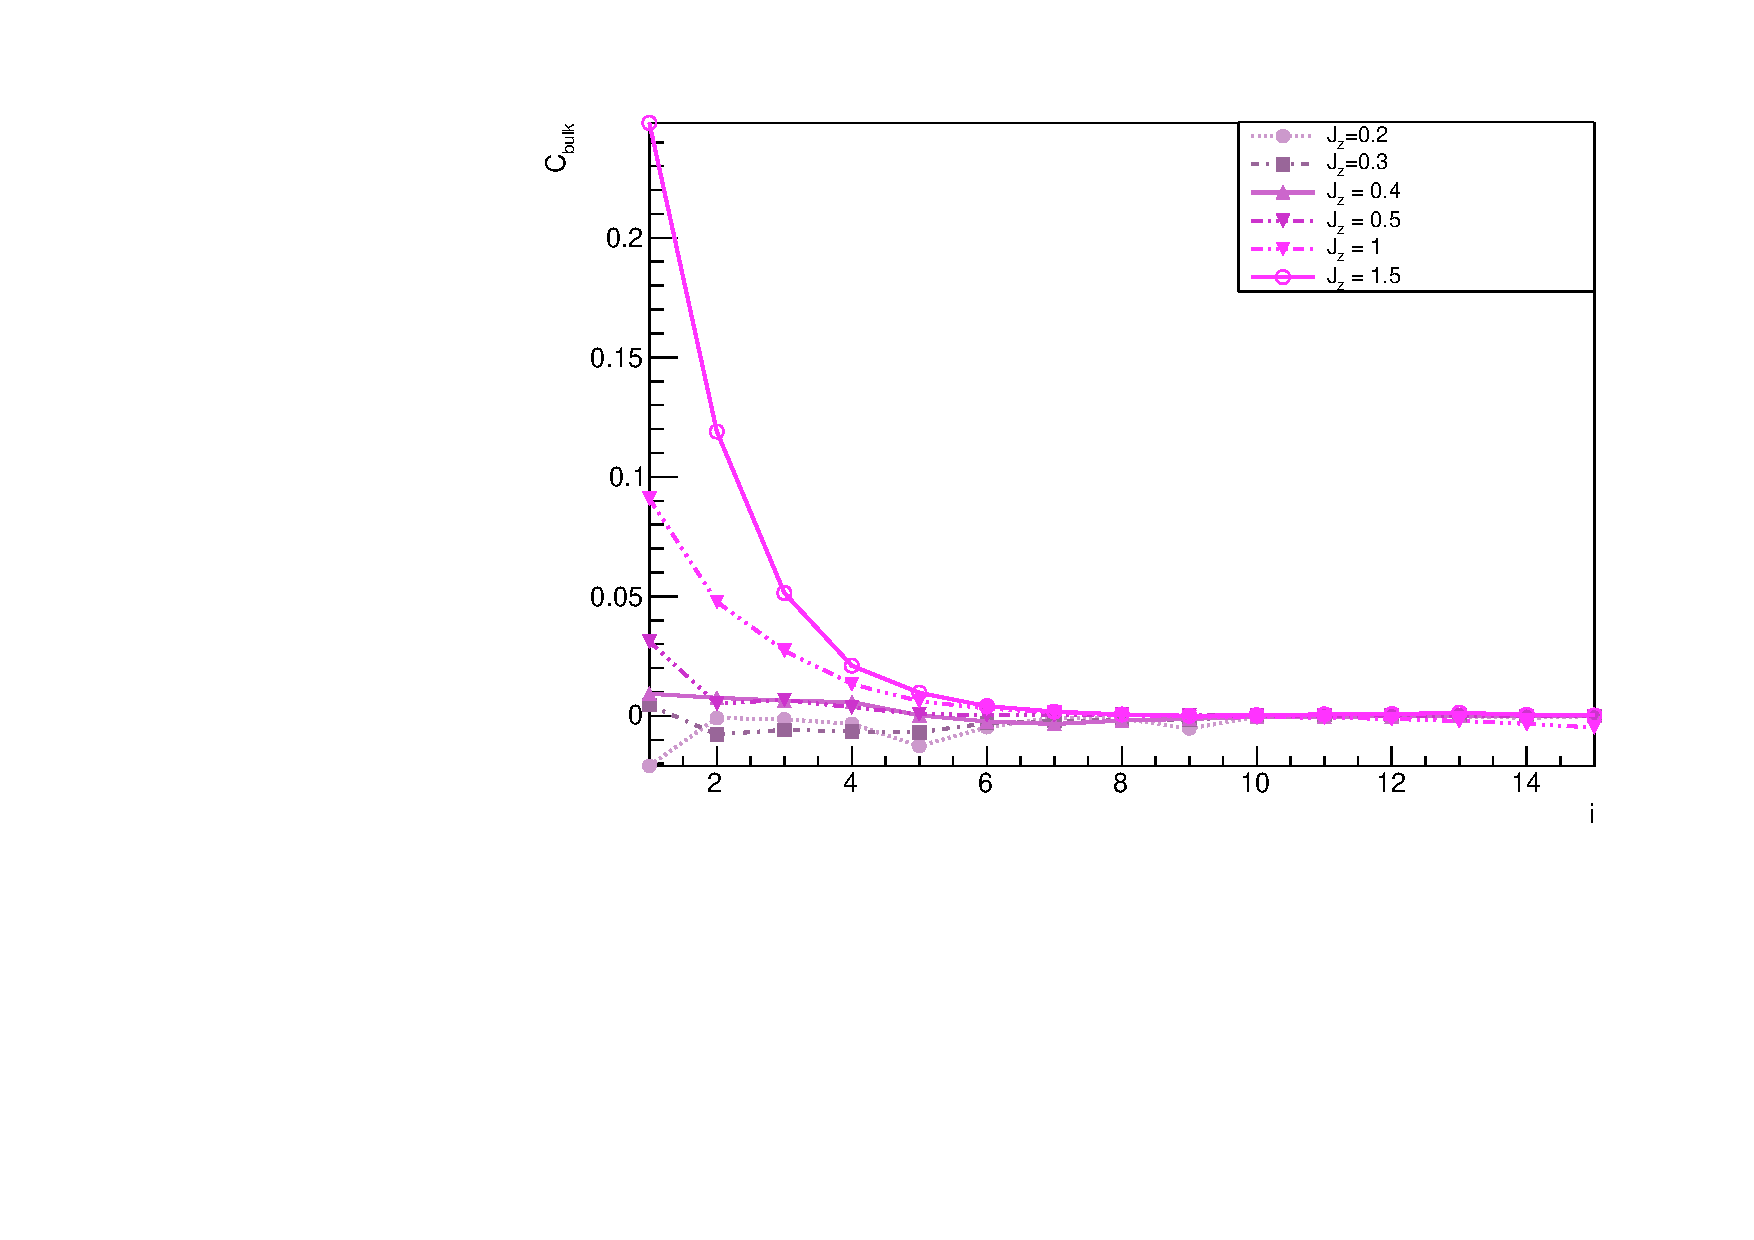
\includegraphics[scale=0.7]{Figures/16sites/16sites_CFBulkCONNvsJz.pdf}
    \captionsetup{width=1.\linewidth}
    \caption{Correlation function of a 16-sites chain, with $\gamma = 1$ for several values of $J_z$. Data obtained from MPO method.}
    \label{fig:16sites_CFBulkCONNvsJz}
\end{figure}

The two-point correlation function, displayed in fig.~\ref{fig:16sites_CFBulkCONNvsJz}, for $J_z \geq 0.5$ shows a behaviour similar to that seen in the previous chapter, with an exponential profile of the correlation function. In this case, however, there is a discontinuity in its behaviour for $J_z < 0.5$. Indeed, the plots show a null correlation function for such values of $J_z$, trend that is consistent with the profile of spin current in fig.~\ref{fig:16sites_SpinCurrVaryingJz}.